\begin{frame}
    \frametitle{Genetischer Algorithmus}
    \begin{itemize}
      \item unendlich viele Möglichkeiten
      \item Lösung sind bekannt.
      \item Trainingsdaten vorhanden
      \item Später einfacher Regeln zu erstellen.
    \end{itemize}
\end{frame}

\begin{frame}
  \frametitle{Coverage}
  \begin{center}
  \huge{GA Coverage = 73,1 \%}
  \end{center}
  \begin{center}
  \huge{Human Coverage = 74,6 \%}
  \end{center}
\end{frame}


\begin{frame}
    \frametitle{App um mehr Daten zu bekommen}
    \begin{itemize}
      \item Hoffnung auf mehr Testdaten
      \item Direkter Nutzen für beteiligte Personen
      \item Nie über alpha-stadium hinaus gekommen
      \item Open Source, also fühlt euch frei.
    \end{itemize}
\end{frame}

\begin{frame}
  \frametitle{Startbildschirm}
  \Wider{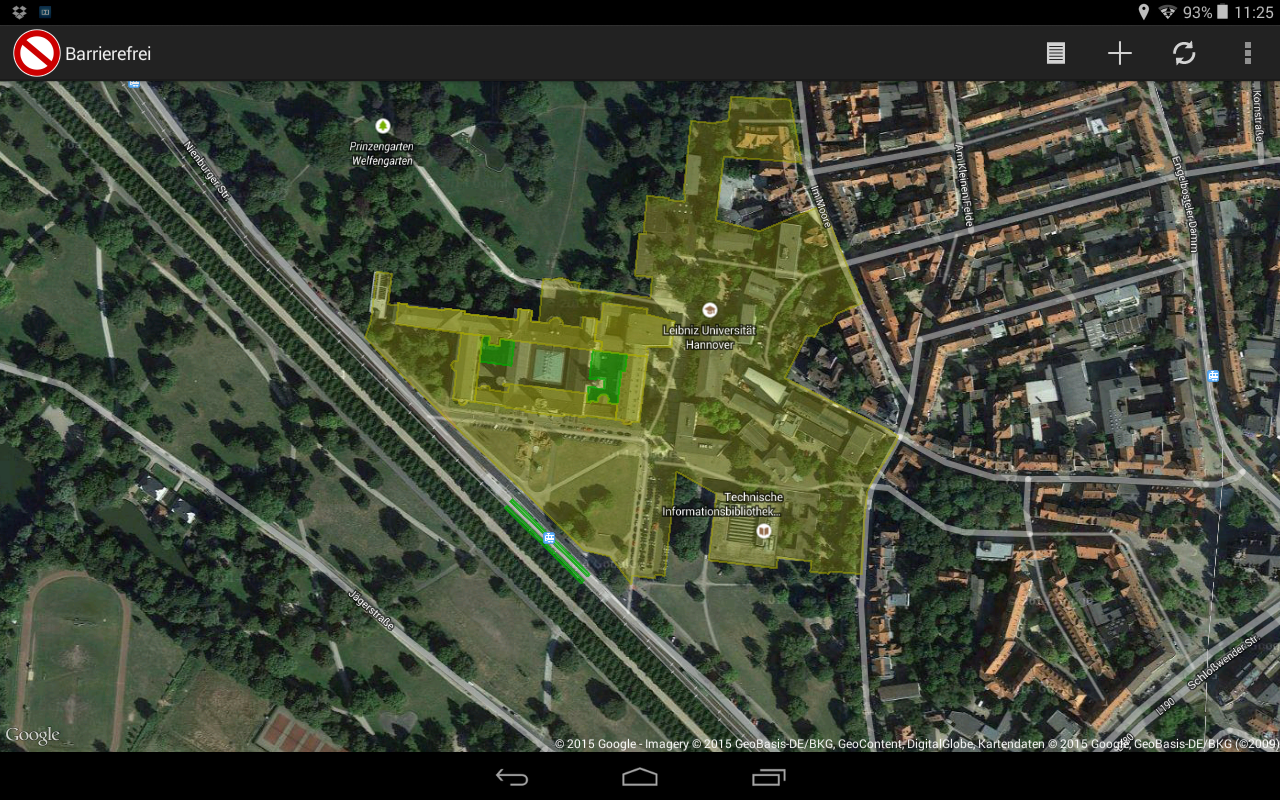
\includegraphics[width=\textwidth]{App_show}}
\end{frame}

\begin{frame}
  \frametitle{Tags}
  \Wider{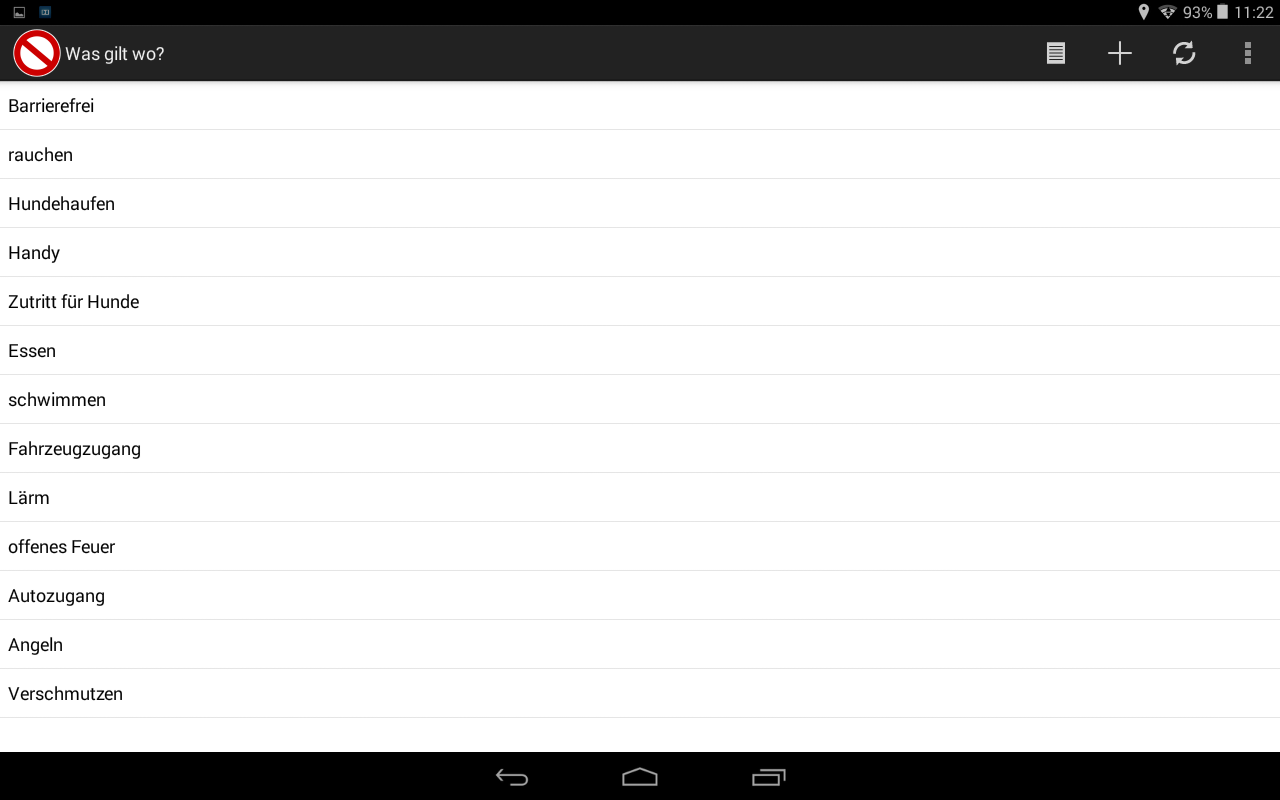
\includegraphics[width=\textwidth]{App_tags}}
\end{frame}

\begin{frame}
  \frametitle{Fläche auswählen}
  \Wider{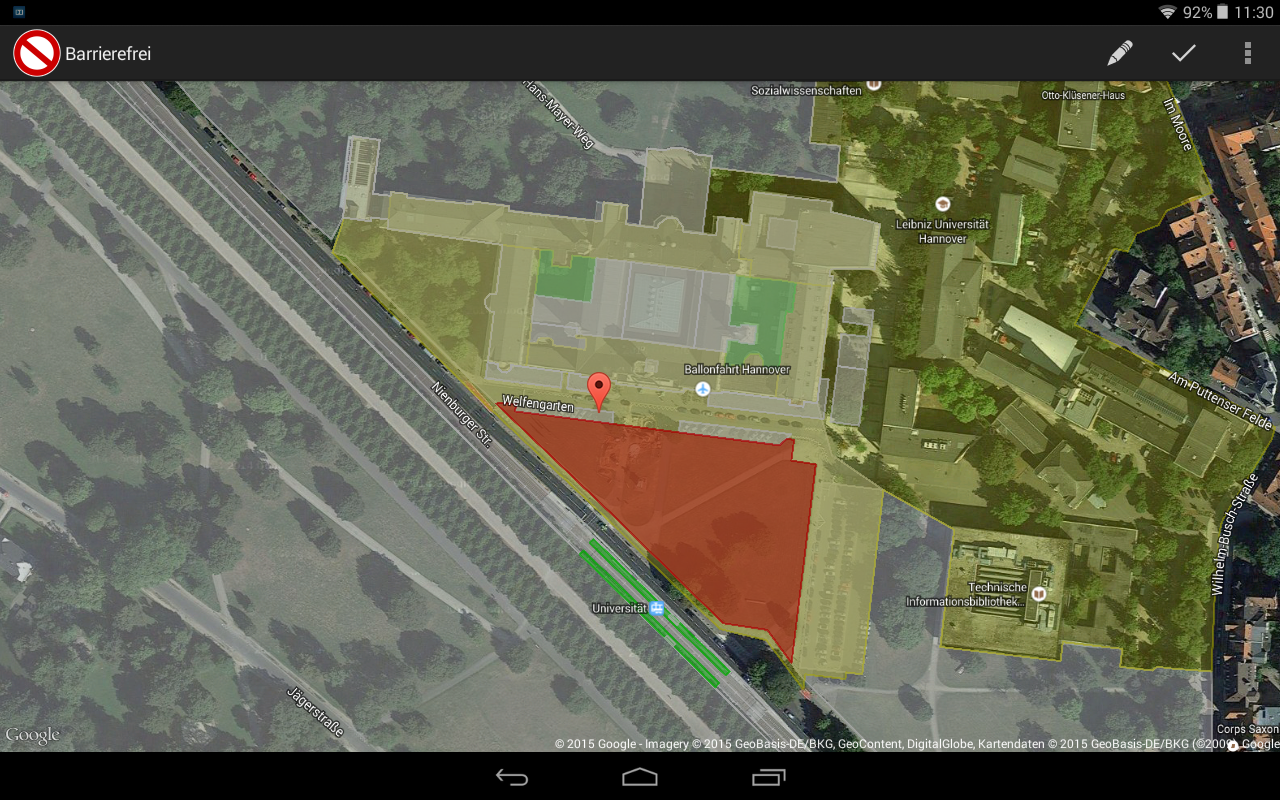
\includegraphics[width=\textwidth]{App_select}}
\end{frame}

\begin{frame}
  \frametitle{Frei einzeichnen}
  \Wider{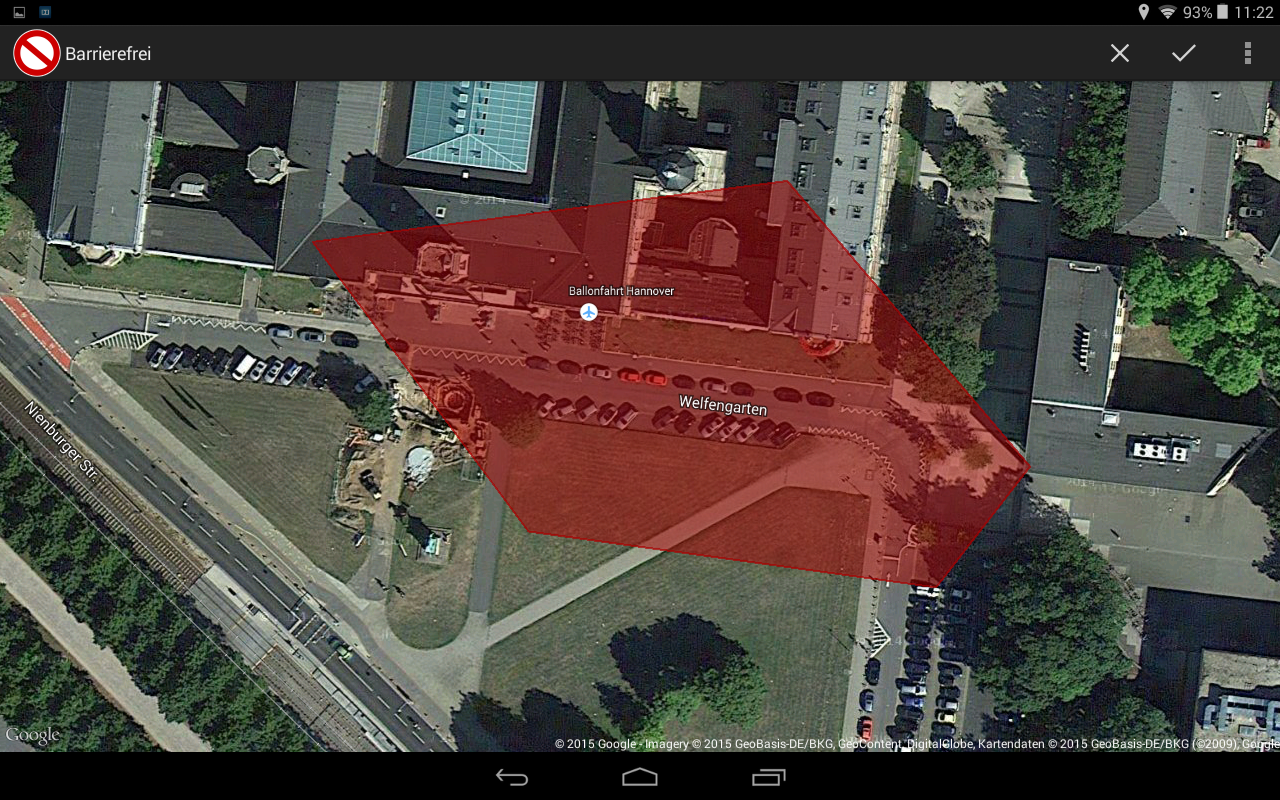
\includegraphics[width=\textwidth]{App_free}}
\end{frame}
